\chapter{Conception}

\section{Dataset}
For this projects, the "SpeechCommands"\cite{warden2018speech} dataset will be used. This dataset was created by Pete Warden, 
working for Google, with the intent of creating a fundamental set of simple commands spoken in English with a lot of variance. 
The data was gather publicly and thus contains audio from different speakers with normal day-to-day audio quality and possibly even background noise. 
Even though the data comes from a public source, its correctness was checked manually and with various alghorhithms to remove too quiet or interrupted words. 
In total, the data contains 105.829 audio files (3.4 GB) for 35 words spoken by 2.618 different people. All audio files are exacly one seconds long and the data is alligned 
so that words all start and end roughly at the same time. The audio comes in the WAVE format with 16bit single channel (mono) values, sampled at a rate of 16kHz.
The dataset also contains audio files containing common background noise, that can be used for evaluation. The dataset is split into multiple subsets for 
training, testing and validation, specified by specific file lists in the same folder.

\section{Model} \label{model}
The model will be a deep convolutional neural network with 5 convolutional layers described as M5 \cite{dai2016deep}. This was choses as they claim a reasonable high accurary of
over 60% in a 10 class audio classification with a training time of a minute per epoch. They use a very high sampling rate of 32kHz and a very aggresive reduction of the temporal
resolution in the first layer with a kernel size (or receptive field) of 80, a stride of 4 and a ouput size of 128. After each layer, a batch normalization
and a maxpooling of size 4 is performed, further reducing the feature maps. After the first layer, the kernel size is reduced to a more normal size of 3 and the stride reduced to 1.
The heavy reduction of resolution is complemented by a doubling of the amount of filters each layer. They use ReLU as the activation function. While most classification
problems use multiple connected layers after the convolutional layers, the authors claim to use a "fully convolutional design" without fully connected layers. Instead, they
use a global average pooling to reduce the feature maps to a single dimension. At the end, a softmax function is applied.

\section{Audio Capture} \label{audio_capture}
As the quality should be evaluated with a real microphone, the \texttt{audio_capture} ROS package is used for this project. It can be started as a ROS node
and exposes the two topics \texttt{/audio} and \texttt{/audio_info}. The first contains the raw audio data as unsigned 8 bit arrays, the second contains metadata about
how the data should be interpreted. Concretly, it contains the number of channels, the sample rate, the bitrate, the sample format and the encoding format.
How the data correlates to the sampled data is controlled via the encoding format (e.g. 16LE means that two bytes in the little endian format make up one sample).
The data for each channel is stored in an interleaved format and contains no header information. The sample rate specifies how often the analog audio signal from
the microphone is converted to a digital signal. The higher it is, the better the quality (e.g. CD audio is sampled at 44kHz). Of couse, the bit rate, 
mainly specified in kilo bits per second (kbps), has to be high enough to allow for that amount of information to be processed, otherwise the higher sample rate is nullified. 
For uncompressed audio, the bit rate can be calculated by multiplying sample rate, byte count per sample and number of channels.

\section{Evaluation Architecture}
The evaluation architecture will be developed as a ROS application as it helps with development and models a potential real world use case as close as possible. 
The following image shows a graph of the architecture and how the nodes interact with each other.

\begin{figure}
  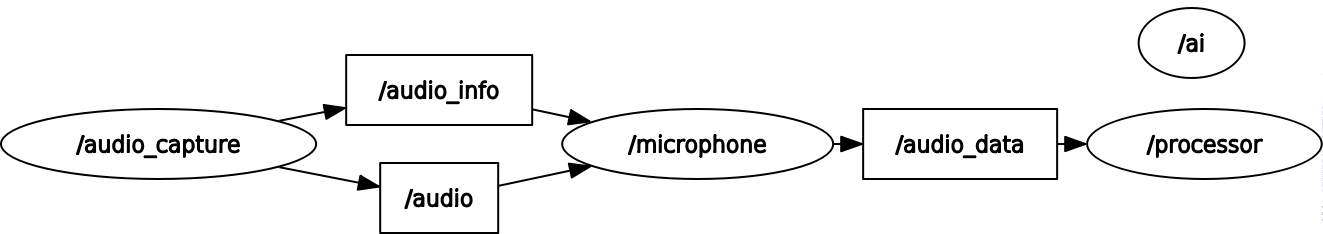
\includegraphics[width=\linewidth]{rosgraph.png}
  \caption{ROS architecture}
  \label{fig:rosgraph}
\end{figure}

As described in section \ref{audio_capture}, the raw audio data and metadata get sent to two topics that are subscribed by the microphone node. It is responsible 
for recording the data when a specific user input has been made. Once another input was made, the data has to be aggregated and sent to the \texttt{audio_data} topic. It is 
subscribed by the processor node, which handles the necessary conversions so that it is compatible with the input of the model. It then also invokes the ai service
which predicts the command and sends it back, together with the probability. To do that, the ai node has to load the pretrained model and metadata about the
used model like the labels it can predict and the used sample rate. The predicted command will then be shown on the console for now.
